

\documentclass[conference]{IEEEtran}

\usepackage{adjustbox}
\usepackage{graphicx}
\usepackage{alphalph}

\let\OLDitemize\itemize
\renewcommand\itemize{\OLDitemize\addtolength{\itemsep}{1em}}
\let\OLDenumerate\enumerate
\renewcommand\enumerate{\OLDenumerate\addtolength{\itemsep}{1em}}
\renewcommand\thesubsectiondis{\AlphAlph{\value{subsection}}.}% for the headings in the text
\renewcommand\thesubsection{\mbox{\thesection-\AlphAlph{\value{subsection}}}}% for the ToC, for example     


% correct bad hyphenation here
\hyphenation{op-tical net-works semi-conduc-tor}


\begin{document}

\title{Assignment Helper\\ Empowering Your Programming Skill \\ Power OVERWHELMING co.}

% author names and affiliations
% use a multiple column layout for up to three different
% affiliations
% \author{\IEEEauthorblockN{Jae-gook Kim}
% \IEEEauthorblockA{Department of Information System\\
% Hanyang University, Seoul,  Korea\\
% Email: claretta@hanyang.ac.kr}
% \and
% \IEEEauthorblockN{Kyung-min Kim}
% \IEEEauthorblockA{Department of Information System\\
% Hanyang University, Seoul,  Korea\\
% Email: kimkmhk@hanyang.ac.kr}
% \IEEEauthorblockN{Ji-hoon Lee}
% \IEEEauthorblockA{Department of Finance,\\ Business School,\\
% Hanyang University, Seoul,  Korea\\
% Email: 1equal2@hanyang.ac.kr}
% \and
% \IEEEauthorblockN{Kyo-ho Lee}
% \IEEEauthorblockA{Department of Information System\\
% Hanyang University, Seoul,  Korea\\
% Email: 1equal2@hanyang.ac.kr}}


% conference papers do not typically use \thanks and this command
% is locked out in conference mode. If really needed, such as for
% the acknowledgment of grants, issue a \IEEEoverridecommandlockouts
% after \documentclass

% for over three affiliations, or if they all won't fit within the width
% of the page, use this alternative format:
% 
\author{\IEEEauthorblockN{Ji-hoon Lee\IEEEauthorrefmark{1},
Jae-gook Kim\IEEEauthorrefmark{2},
Kyung-min Kim\IEEEauthorrefmark{3}, and
Kyo-ho Lee\IEEEauthorrefmark{4} }
\IEEEauthorblockA{\IEEEauthorrefmark{2}\IEEEauthorrefmark{3}\IEEEauthorrefmark{4}Department of Information System}
\IEEEauthorblockA{\IEEEauthorrefmark{1}Department of Finance, Business School}
\IEEEauthorblockA{Hanyang University, Seoul, Korea}
\IEEEauthorblockA{Email: \IEEEauthorrefmark{1}starypoc@hanyang.ac.kr,  \IEEEauthorrefmark{2}claretta@hanyang.ac.kr, \IEEEauthorrefmark{3}kimkmhk@hanyang.ac.kr, \IEEEauthorrefmark{4}1equal2@hanyang.ac.kr}}



\maketitle

\begin{abstract}
Assignment Helper is a program to help people who have difficulties with their programming language assignments. Assignment Helper will able to help the assignment by crawling the data from webs such as programmer forums and then find similar questions and related codes. It will also have a verification function and will check the codes by using CRC or other compilers. It shall check it by testing the input, output and the expectation all together.

\centering


\begin{table}[h]
\renewcommand{\arraystretch}{1.3}
\caption{Role Assignment}
\label{table_role}
\centering
\begin{adjustbox}{width=0.5\textwidth}
\small
\begin{tabular}{c||c||c}
\hline
\bfseries Role & \bfseries Name & \bfseries Task Description \\
\hline\hline
Developer Manager  & Kim Jae-gook & \parbox[t]{5cm}{Managing whole process of developing\\ the program. }\\
\hline
Users & Lee Ji-hoon & \parbox[t]{5cm}{Seeking for the usefulness compare\\ to other similar programs.}\\
\hline
Cutomers & Kim Kyung-min & \parbox[t]{5cm}{Finding out whether the project is \\ valuable.}\\
\hline
Developer & Lee Kyu-ho & \parbox[t]{5cm}{Implementing the program.}\\
\hline

\end{tabular}
\end{adjustbox}

\end{table}
\end{abstract}

\IEEEpeerreviewmaketitle


\section{Introduction}

\subsection{Motivation}
We have started this project with the motivation to help students (especially freshman) who are struggling with their assignments. Other assignments like history or natural science can easily find their assignment sources quickly from just googling it simply. However, it is impossible to do that simple procedure in programming language assignment. Without perfect knowledge about the computer languages, it comes out difficult to solve their programming language assignment. 

We discussed about a solution to solve this. We concluded that it is not easy to study programming languages especially to the students who studied only at school and have never lived closed to computer languages; The students who only studied subjects for KSAT, the entrance exam for university!

\subsection{Problem Statement}
It is problematic for those who first met the programming language and getting no additional help. It can be not only unfair but also can cause inefficiency in terms of the social resource allocation. Maybe, some novice students might have natural talents at computer programming. But others needs opportunities to catch up. So, we are going to build a program to ease the life of these novice students.


\subsection{Research on Any Related Software}
Our program aims for helping students who is unfamiliar with programming paradigms. There are some services which provide help to those students in primitive levels than our service.

\subsubsection{Education Service: Scratch}
There are many programs for teaching programing language, but Scratch is the most representative one. Scratch does not execute commands by entering code with long instructions. Instead, click and drag the block to move the feature to perform the command. Scratch is a popular child-coding tool for schools and institutions worldwide. Scratch's intuitive interface is useful but has difficulty to find right answer. If one wants to make a program working properly. He should keep try until it matches. It is very frustrating for those who want to know the correct answer right away.

\subsubsection{Easier Coding: Emmet}
Emmet is a programming language that makes it easy to write CSS, even though it can save your coding time, the language you should learn for one programming language increases. Also, if you are not aware of the language, it is hard to get used to it. Instead, Assignment Helper will provide the coding style with natural language processing.

\subsubsection{Crowdsourcing and Knowledge Sharing: Stackoverflow}
Stackoverflow is a site where programmers ask and answers about programming. Stackoverflow is the largest developer community on the scale. It will be a good idea to ask questions here for the answers comes up very quickly.
Since there are a lot of questions that has been answered, the problems that you need answers are mostly up on the forum already. In other words, rather than asking, you are more likely to search and get answers. But the point is for the beginners, it can even be hard to determine what to find. You must define the search keywords yourself. It would be a big hurdle for beginners. The limitation is that there is no recommend keywords.

\subsection{Distinguishable Features of Assignment Helper} % (fold)
\label{sub:distinguishable_features_of_assignment_helper}
There are countless amounts of services that tries to help the problem we defined. Our Assignment Helper will have differentiating features from existing services. Some distinguishable features are as follows:

\subsubsection{Lightening The Burden On Determining Search Keywords}
For some questions for beginners, it could be hard to determine a search keyword by themselves. For example, if they want to know what list object can 'do', it is appropriate to google on 'list method in python'. To google the word 'method', the user should know the word beforehand, which is practically impossible without any additional help.


Assignment Helper will allow to search on more natural-language-like queries, making the user easy to search with their actual thoughts.

\subsubsection{Grouping Related Questions}
With natural-language-like queries, it could be hard to guess what the user intended from the very beginning. Assignment Helper will explore broad range of possibilities and suggest each to the users.

\subsubsection{Getting the Working Codes Right Away from the Internet}
There are numerous codes that are floating on the internet. But it is not verified whether the codes on the internet works properly or not. Assignment Helper will check the validity of the code automatically 

% subsection distinguishable_features_of_assignment_helper (end)

\section{Requirements} % (fold)
\label{sec:requirements}


\textit{\textbf{Frontend Related}}

\subsection{Building installation Manual}
\textit{ }

\subsection{Building Web-like Client}
\textit{ }

\subsection{Instruction for Users}
\begin{itemize}
  \item Description
\end{itemize}
\textit{ }

\subsection{Building Search and Select UI}
\begin{itemize}
  \item Textbox for a query
  \item Cardbox to code select and check
  \begin{itemize}
    \item Checkbox for choosing code
  \end{itemize}
  \item Expandability
  \begin{itemize}
    \item Can scroll infinitely (like Facebook) in case there are lot of result
  \end{itemize}
  \item Show result code
  \begin{itemize}
    \item Textbox for code lines
  \end{itemize}
\end{itemize}
\textit{ }

\subsection{Checking Code Validity}
\begin{itemize}
  \item Let users know the validity of the codes
\end{itemize}
\textit{ }

\subsection{Providing Information Security}
\begin{itemize}
  \item Prevent from user clicking the button twice
  \item Immediate response to button can make system overload
\end{itemize}
\textit{ }


\textit{\textbf{Backend Related}}
\textit{ }


\subsection{Search Query Processing}
\begin{itemize}
  \item Natural Language Processing Technique
  \begin{itemize}
    \item Understanding the input with NLP
  \end{itemize}
  \item DB for search keyword
  \begin{itemize}
    \item Collecting keywords for seraching codes in DB to maximize accuracies
  \end{itemize}
  \item Function to extract keyword from input comparing to DB for search keyword
\end{itemize}
\textit{ }

\subsection{Learning System for Maximizing Accuracy}
\begin{itemize}
  \item Collect data from user and get feedback from them
\end{itemize}
\textit{ }

\subsection{Crawling and Parsing}
\begin{itemize}
  \item Crawling data from website like programmer forum
  \item Parsing program codes
  \begin{itemize}
    \item Parsing the codes using keywords for finding start-end point
    \item ex) including <iostream>, return 0 in c++
  \end{itemize}
\end{itemize}
\textit{ }

\subsection{Grammar Check}
\begin{itemize}
  \item DB for grammar rules
  \begin{itemize}
    \item Building rules for testing the codes wheter valid or not
  \end{itemize}
  \item Algorithm to check the grammar
\end{itemize}
\textit{ }

\subsection{Testing Compile}
  \begin{itemize}
    \item Compiling searched codes using CRC
  \end{itemize}
\textit{ }

\section{DEVELOPMENT ENVIRONMENT} % (fold)
\label{sec:development_environment}
\subsection{Choice of Software Development Platform} % (fold)
\label{sub:choice_of_software_development_platform}

\begin{enumerate}
  \item Operating System
  \begin{itemize}
    \item OS: Windows
    \item Reason: The program aims for students who are not familier with programming. They are highly likely to use Windows and have few knowledge on other platform such as Linux.
  \end{itemize}
  \item Language and Platform
  \begin{itemize}
    \item Language and Platform: Python 3.6 with PyQt4
    \item Reason: Easy to implement crawling and parsing dealing with text segments as well as leaving rooms to use other packages.
  \end{itemize}
\end{enumerate}
\textit{}

% subsection choice_of_software_development_platform (end)

\subsection{Software in Use} % (fold)
\label{sub:software_in_use}

\begin{enumerate}
  \item \textit{Sublime Text 3}: Text editor for general use
  \item \textit{qt designer 4.12}: GUI based GUI designer for Qt environment
  \item \textit{pyCharm}: genral IDE for Python
  \item \textit{pandas}: Python package to deal with datas
  \item \textit{PyQt4}: Python package to deal with Qt gui
  \item \textit{stackexchage REST API}: REST API to do stack overflow search and get datas
  \item \textit{beautifulsoup4}: Python package for parsing XML and HTML
  \item \textit{requests}: Python package that assists to issue an HTML Request
  \item \textit{gcc}: C compiler to verify given source codes
\end{enumerate}
\textit{}
% subsection software_in_use (end)
% section development_environment (end)


\section{SPECIFICATIONS} % (fold)
\label{sec:specifications}

\textbf{Getting Started}

\subsection{Setting - Easy Installation}

\begin{enumerate}
  \item Description
  \begin{itemize}
    \item Executable without installation to facilitate ease of use
    \item Works like portable utility
    \item Basic files only provide barebone program
    \begin{itemize}
      \item Programming language to search need be installed later
    \end{itemize}
  \end{itemize}
  \item Process(or I/O)
  \begin{enumerate}
    \item Download files from website
  \end{enumerate}
\end{enumerate}


\textit{}

\subsection{Setting - Configuration Window}

\begin{enumerate}
  \item Description
  \begin{itemize}
    \item Basic program is not able to use without installing programming language
    \item Provide check window
    \begin{itemize} 
      \item Check each window to install a language pack for a certain language 
    \end{itemize}
  \end{itemize}
  \item Process(or I/O)
  \begin{enumerate}
    \item Input: Opening conf.exe
    \item Output: Show conf.exe
  \end{enumerate}
\end{enumerate}

\textit{}

\subsection{Setting - Installing Language Pack}
\begin{enumerate}
  \item Description
  \begin{itemize}
    \item Basic program is not able to use without installing programming language
    \item Provide check window
    \begin{itemize}
      \item Check each window to install a language pack for a certain language 
    \end{itemize}
  \end{itemize}
  \item Process(or I/O)
  \begin{enumerate}
    \item Input: Selecting language packs and proceed 
    \item Output: Pack install on the hard disk
  \end{enumerate}
\end{enumerate}


\textit{}
\subsection{Instruction - README}
\begin{enumerate}
  \item Description
  \begin{itemize}
    \item Provide README file to give basic instruction
  \end{itemize}
  \item Process(or I/O)
  \begin{enumerate}
    \item N/A
  \end{enumerate}
\end{enumerate}


\textit{}

\subsection{Instruction - Basic Tutorial}
\begin{enumerate}
  \item Description
  \begin{itemize}
    \item Give demo-like tutorial on the very first run
  \end{itemize}
  \item Process(or I/O)
  \begin{enumerate}
    \item Input: Clicking tutorial on main window
    \item Input2: Initial program execution
    \item Output: Install selected pack on the hard disk
  \end{enumerate}
\end{enumerate}


\textit{}

\subsection{Instruction - On the Fly}
\begin{enumerate}
  \item Description
  \begin{itemize}
    \item Give tooltips on buttons
  \end{itemize}
  \item Process(or I/O)
  \begin{enumerate}
    \item Input: Hovering on a button for 3 seconds
    \item Output: Show up a tool tip
  \end{enumerate}
\end{enumerate}

\textit{}

\textbf{Execution}

\subsection{Execution}
\begin{enumerate}
  \item Description
  \begin{itemize}
    \item Executing the main program
  \end{itemize}
  \item Process(or I/O)
  \begin{enumerate}
    \item Opening the main program(helper.exe)
    \item Program(Process1. UI) shows up within 1 minute
  \end{enumerate}
\end{enumerate}

\textit{}

\subsection{Closing Whole Program}
\begin{enumerate}
  \item Description
  \begin{itemize}
    \item Closing Whole Program
  \end{itemize}
  \item Process(or I/O)
  \begin{enumerate}
    \item Clicking X window on search UI
    \item Program closing
  \end{enumerate}
\end{enumerate}

%프롬프트
\textit{}

\textbf{Process 1. Searching}

\subsection{Search - UI}


\textit{}

\subsection{Search - History}


\textit{}

\subsection{Search - Option}
%프로그래밍 언어 선택

\textit{}

\subsection{Search - Auto Completion}


\textit{}

\subsection{Request Submission by Key Press}


\textit{}

\subsection{Request Submission by Clicking}


\textit{}

\subsection{Request Submission - Waiting UI}


\textit{}

\subsection{Request Submission - Abort}


\textit{}

\subsection{Request Processing - Extracting Keyword}


\textit{}

\subsection{Request Processing - Crawling(Stackoverflow)}


\textit{}


\subsection{Request Processing - Crawling(Google)}


\textit{}

\subsection{Request Processing - Detect Code Part}


\textit{}
\subsection{Request Completed - UI}


\textit{}

\textbf{Process 2. Code Selction}

\subsection{Code Selection - Basic UI}


\textit{}

\subsection{Auto Compile Test - Requesting}


\textit{}

\subsection{Auto Compile Test - Success}
''color of the code section goes green

\textit{}

\subsection{Auto Compile Test - Failure}


\textit{}

\subsection{Auto Compile Test - Edit Code Snippet}


\textit{}


\subsection{Cancellation(2) - Clicking Return Button}


\textit{}


\subsection{Cancellation(2) - Cliking X Window Button}
''same as clicking return button

\textit{}

\subsection{Selection - Proceed without testing}
%put warning window

\textit{}

\subsection{Prompt - Cancellation}


\textit{}

\subsection{Prompt - Proceed}


\textit{}

\textbf{Process 3. Manual Verification}

\subsection{Manual Verification - UI}


\textit{}

\subsection{Manual Testing - Requesting}


\textit{}

\subsection{Test Processing - Check Compiling}
''check if compiled if compiled use that

\textit{}

\subsection{Manual Testing - Success}
''print output on the output window

\textit{}

\subsection{Manual Testing - Failure}
''print error message on the output window

\textit{}

\subsection{Cancellation(3) - Clicking Return Button}


\textit{}

\subsection{Cancellation(3) - Cliking X Window Button}


\textit{}


\textbf{Process 4. Result Saving}

\subsection{Result - UI}


\textit{}

\subsection{Cancellation(4) - Clicking Return Button}


\textit{}

\subsection{Cancellation(4) - Cliking X Window Button}


\textit{}




''-------------end of the document-------------------''
% figure example --------------
\begin{figure}[h]
\centering
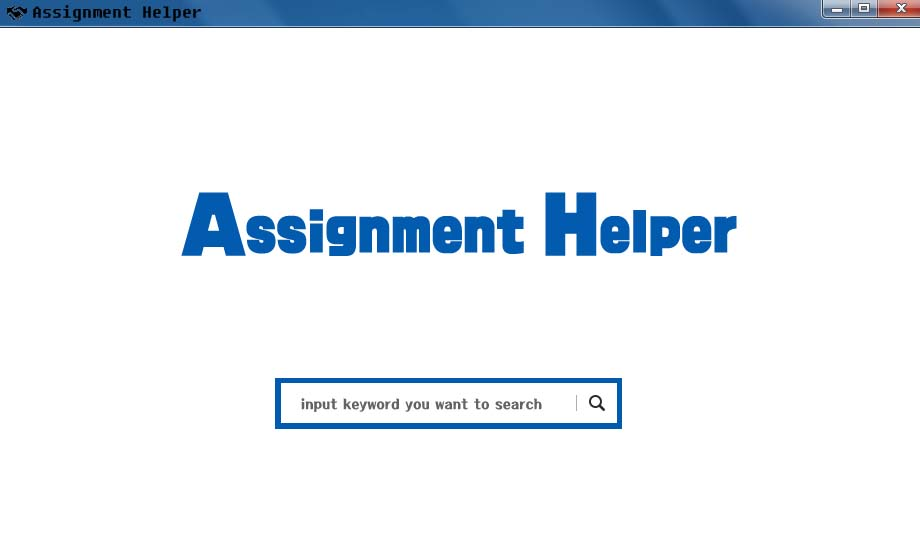
\includegraphics[width=0.5\textwidth]{./figures/UI_main.jpg}
%text slot
\caption{Example Example.}
\label{fig_sim}
\end{figure}

% section specifications (end)
% \begin{thebibliography}{1}

% \bibitem{IEEEhowto:kopka}
% H.~Kopka and P.~W. Daly, \emph{A Guide to \LaTeX}, 3rd~ed.\hskip 1em plus
%   0.5em minus 0.4em\relax Harlow, England: Addison-Wesley, 1999.

% \end{thebibliography}




% that's all folks
\end{document}


